\documentclass[12pt,onecolumn,a4paper]{article}
\usepackage{epsfig,graphicx,subfigure,amsthm,amsmath}
\usepackage{color,xcolor}     
\usepackage{xepersian}
\usepackage{cite}
\usepackage{fontspec}
\usepackage{multirow}

\settextfont[Scale=1]{BMitra}
\setlatintextfont[Scale=0.8]{Vazir-Regular}


\begin{document}
\title{گزارش تکلیف ۵ درس یادگیری ماشین} 
\author{کسرا سینایی\\
شماره دانشجویی ۸۱۰۶۹۶۲۵۴\\
}
\date{\today}
\maketitle
\thispagestyle{empty}
\newpage
\section*{سؤال یک}
\subsection*{الف}
روش‌های جست و جو:
\begin{description}
    \item[$\bullet$] \lr{Exhustive}: در این روش‌ها تمام حالات ممکن برای به دست آوردن زیرمموعه‌ای از فیچرها امکان پذیر است در نظر گرفته می‌شوند. اگر $n$ فیچر داشته باشیم، پیچیدگی محاسباتی این روش $O(n^{2})$ است. به دلیل پیچیدگی محاسباتی بالا، این روش معمولا کاربردهای کمی دارند (مثال: \lr{Breadth First Search})
    \item[$\bullet$] \lr{Heuristic}: روش‌هایی مانند \lr{SFS}، \lr{SBS}، \lr{BDS}  و ... هستند. در این روش‌ها یا با مجموعه‌ی کامل فیچرها شروع کرده و به ترتیب فیچرهایی که حذف آن‌ها بهینه ترین زیرمجموعه جدید را نتیجه دهد حذف می‌شوند، یا با زیرمجوعه تهی از فیچرها شروع کرده و به مرور فیچرهایی را که بهینه ترین زیرمجموعه جدید را حاصل می‌کنند اضافه می‌شوند به زیرمجموعه فیچرها.
    \item[$\bullet$] \lr{Randomize}: در این روش ابتدا به صورت اتفاقی زیرمجموعه‌ای از فیچرها انتخاب می‌شوند، سپس با استفاده از الگوریتم‌هایی مانند ژنتیک، \lr{RGSS} و ... به بهینه سازی تابع هزینه می‌پردازند تا زیرمجموعه بهینه از فیچرها به دست آید.
\end{description}
روش‌های ارزیابی:
\begin{description}
    \item[$\bullet$] \lr{Filter Methods}: این روش‌ها بدون توجه به اللگوریتم طبقه‌بندی زیرمجموعه انتخابی از فیچرها را ارزیابی می‌کنند. معیار اصلی ارزیابی اطلاعات موجود در هر زیرمجموعه از فیچر است. این روش‌ها سریع هستند و تمایل به انتخاب زیر مجموعه‌های بزرگی از فیچرها را داغرند.
    \item[$\bullet$] \lr{Wrpper Methods}: برای ارزیابی زیرمجموعه انتخاب شده از فیچرها، معیارهایی در نظر گرفته می‌شود که به الگوریتم طبقه بندی مربوط است. برای مثال پروسه ارزیابی کیفیت زیرمجموعه فیچر انتخاب شده از دقت آن در پیش بینی تعدادی داده تست استفاده می‌شود. این روش‌ها آهسته هستند اما دقیق تر از \lr{Filter Methods} کار می‌کنند.
\end{description}
\subsection*{ب}
در محاسبات \lr{LDA} لازم است معکوس ماتریس $S_w$ را حساب کرد و سپس مقادیر ویژه و بردارهای ویژه $S_{w}^{-1}S_{b}$ را به دست آورد. با افزایش ابعاد مسئله حجم محاسبات جبری افزایش می‌یابد. همچنین اگر تعداد نمونه‌ها کم باشد ممکن است ماتریس $S_{w}$ سینگولار شود.
\\
در \lr{PCA} نیز باید مقادیر ویژه ماتریس کواریانس نمونه‌ها و بردارهای متناظر با آن‌ها محاسبه شوند تا \lr{PC}ها به دست آیند. اگر ابعاد مسئله زیاد شود علاوه بر حجم محاسباتی مقادیر ویژه امکان کاهش دقت تخمین ماتریس کواریانس هم به وجود می‌آید. یکی از نقاط ضعف \lr{PCA} حساسیت ان به اسکیل فیچرها می‌باشد به همین دلیل نرمال کردن دیتا قبل از اجرای الگوریتم اهمیت ویژه‌ای دارد.
\\

\newpage
\section*{سوال دو}
\begin{figure}[h!]
    \begin{center}
    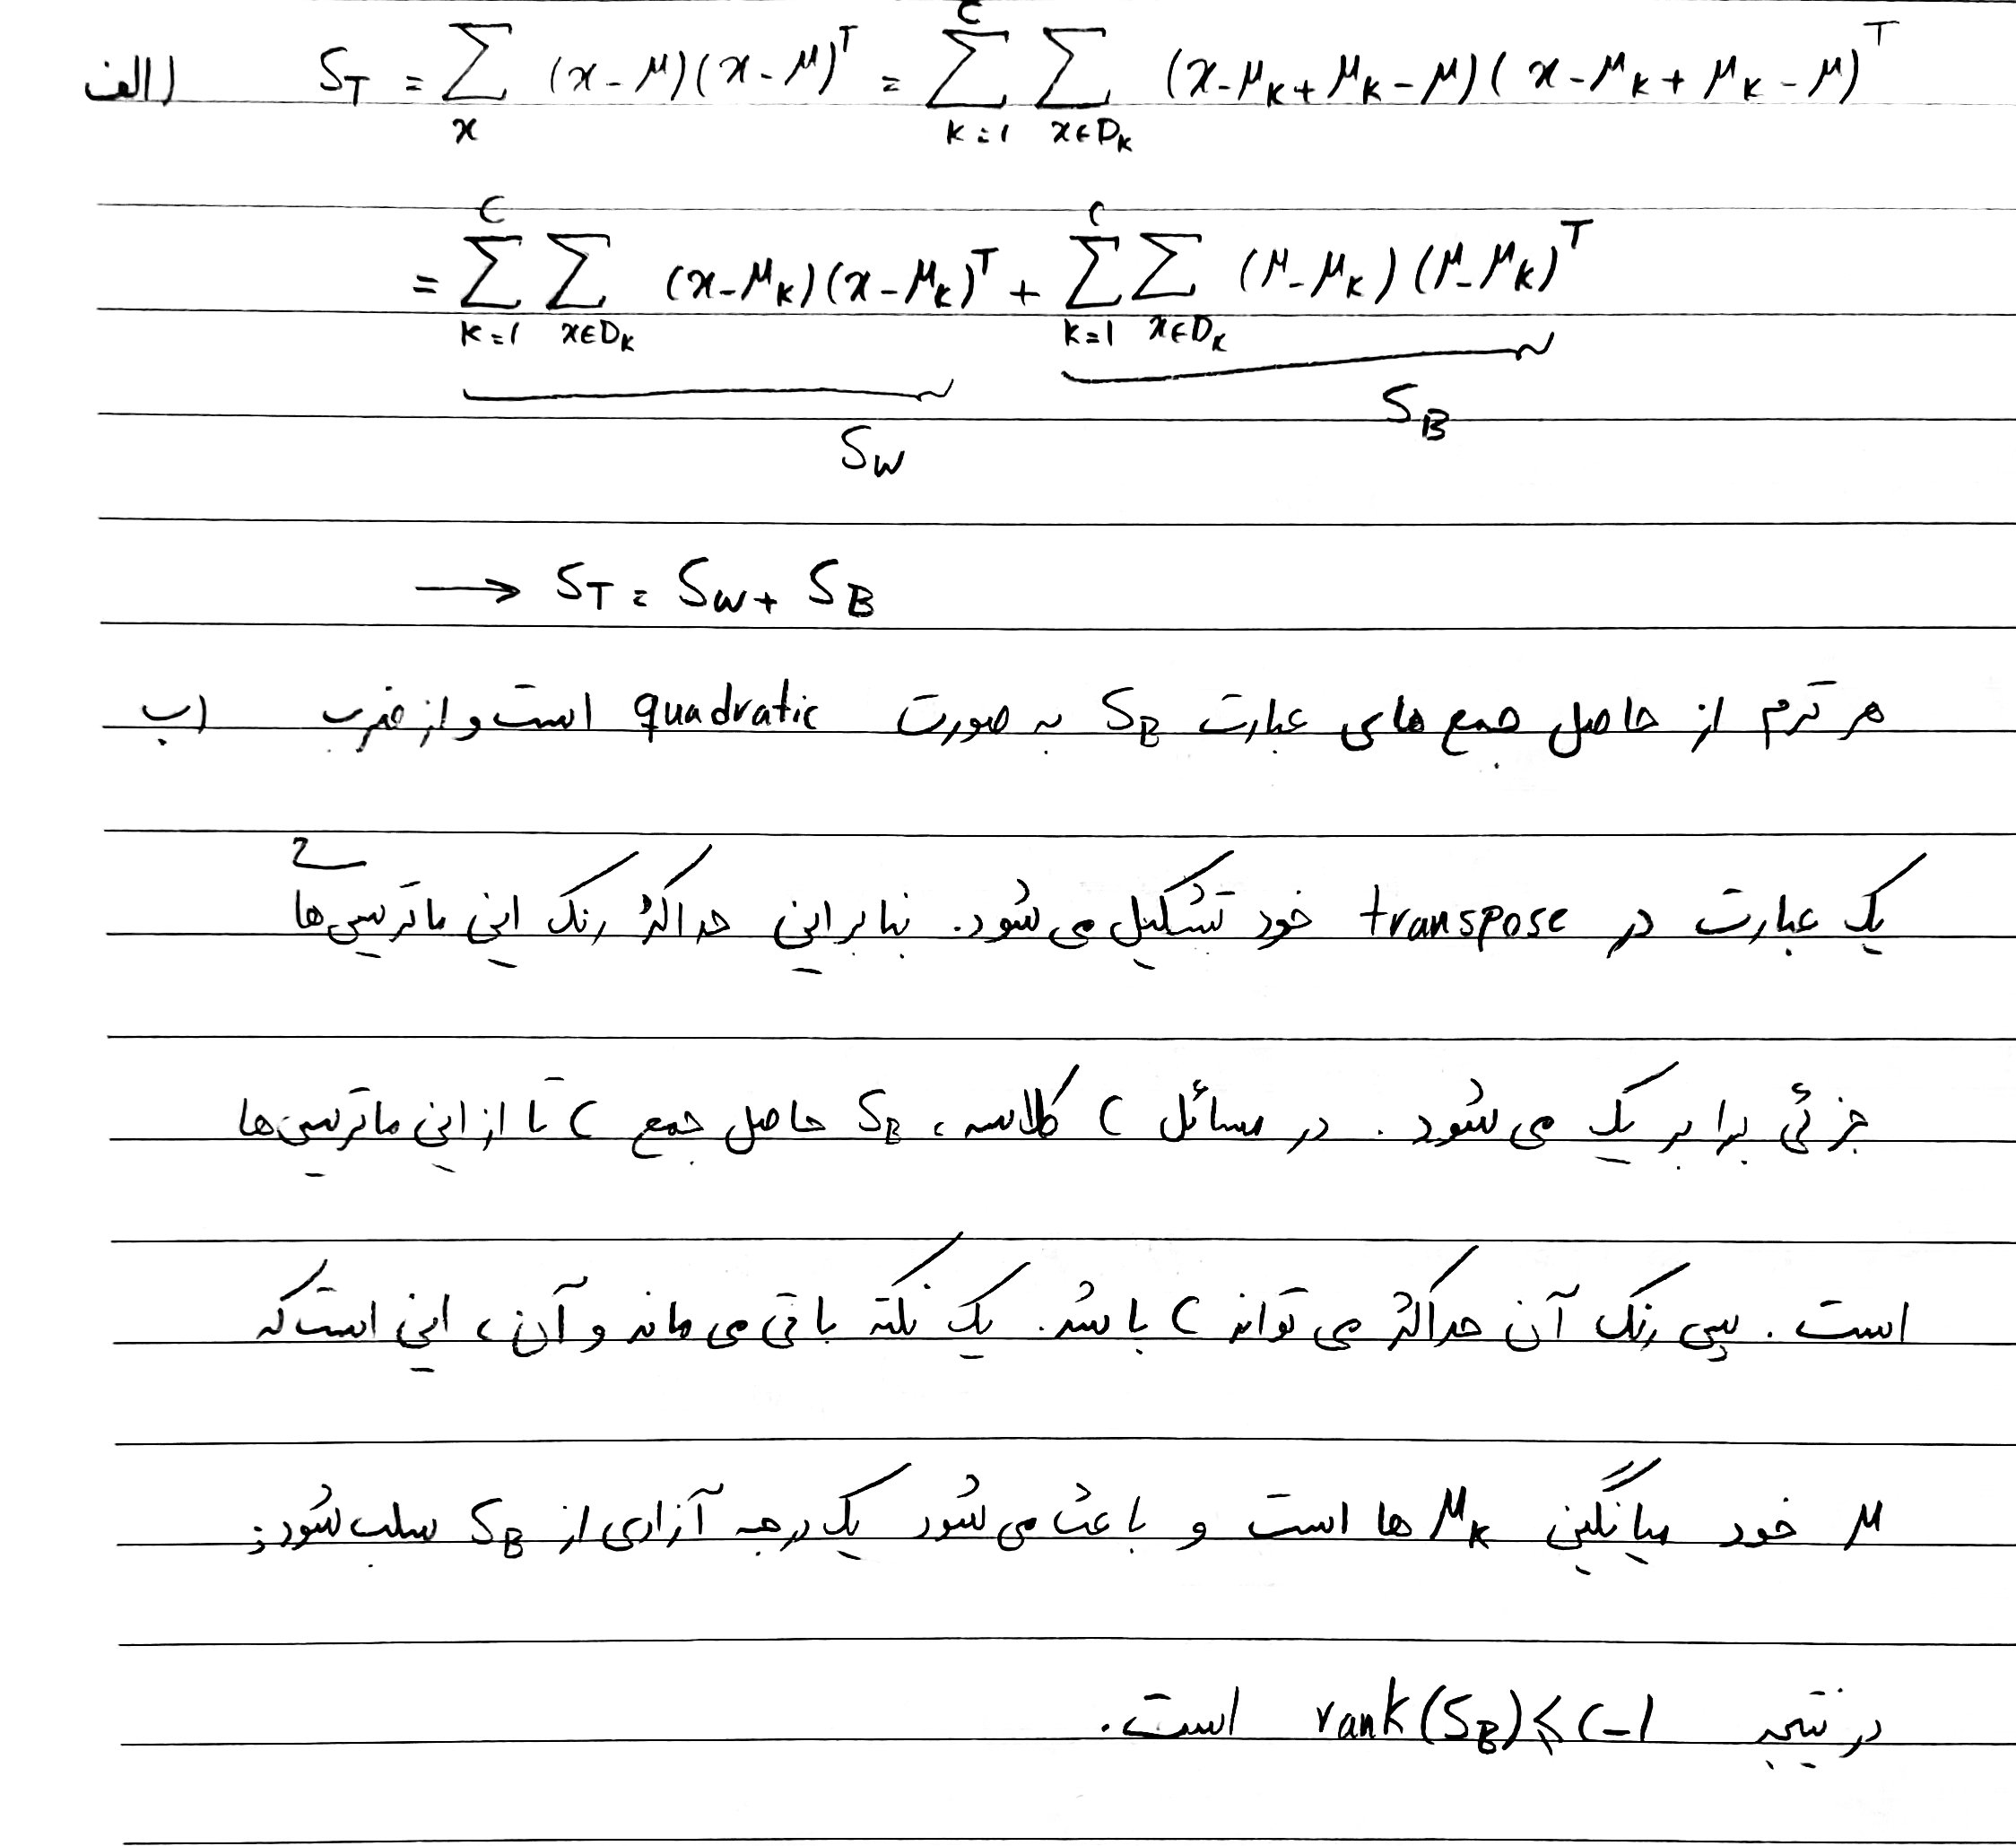
\includegraphics[width=\linewidth]{hand_written/2.jpg}
    \end{center}
\end{figure}

\newpage
\section*{سؤال چهار}
\begin{figure}[h!]
    \begin{center}
    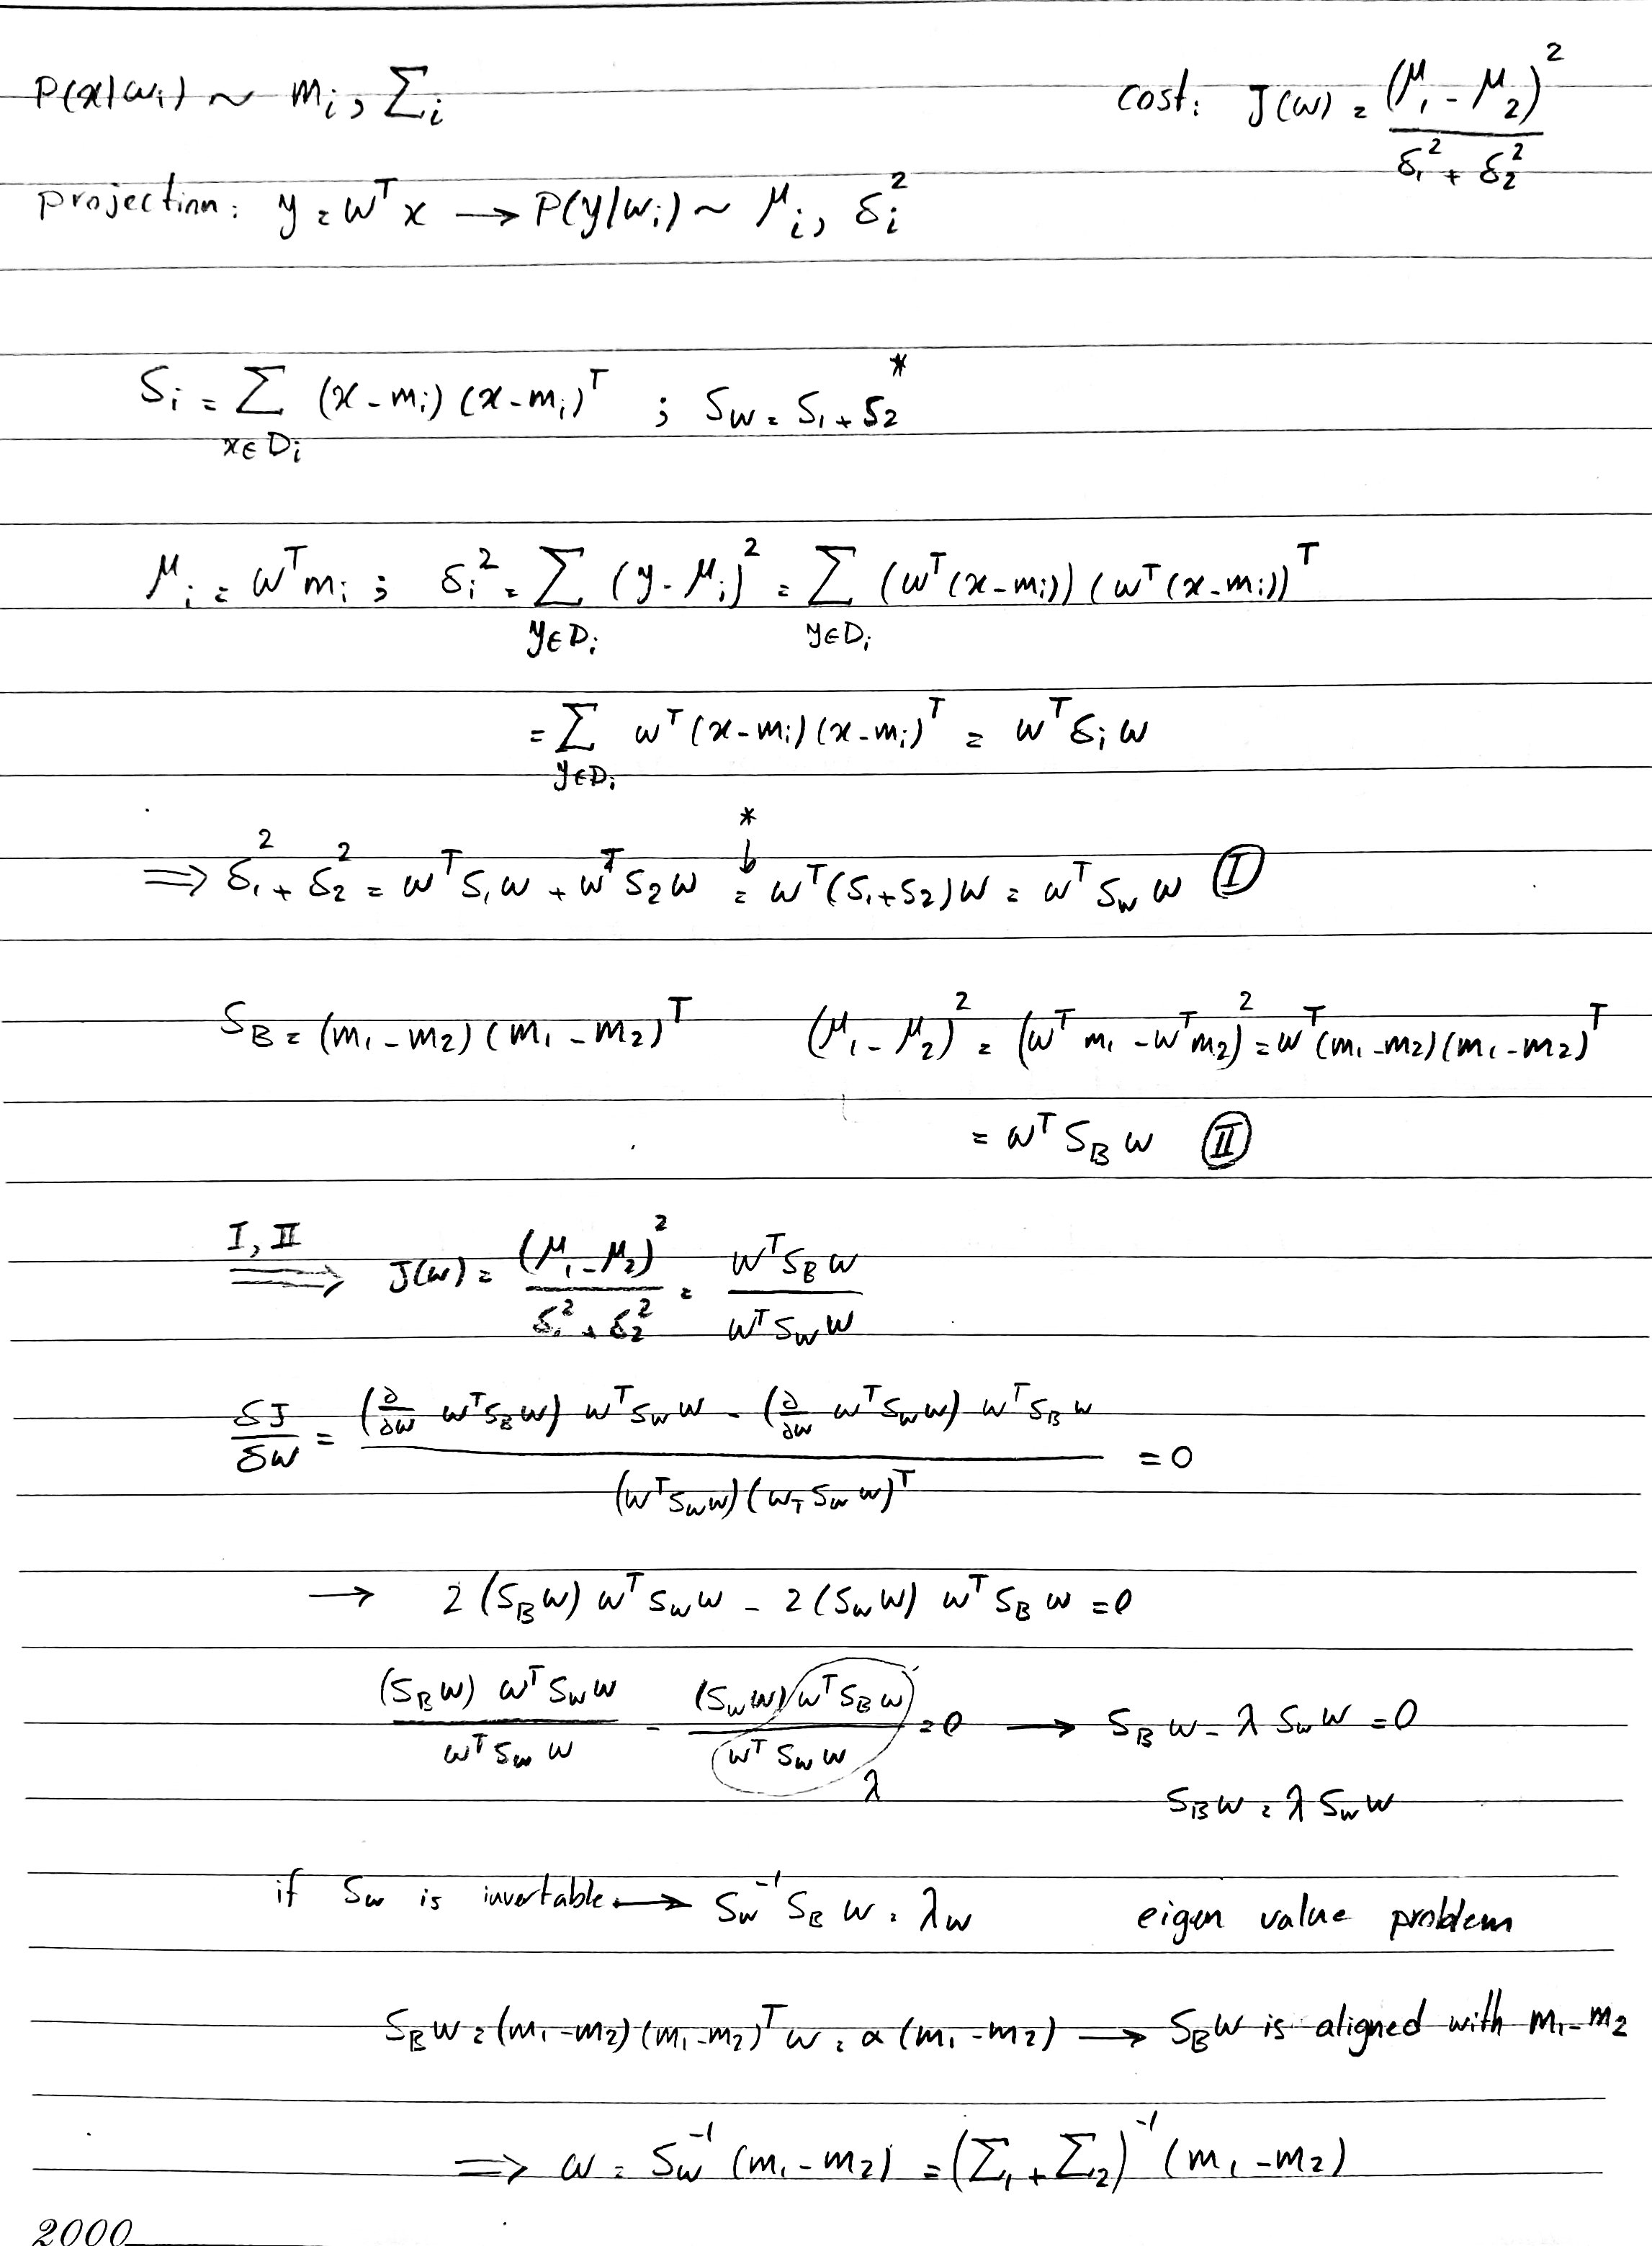
\includegraphics[width=\linewidth]{hand_written/4.jpg}
    \end{center}
\end{figure}

\newpage
\section*{سؤال پنج}
\begin{figure}[h!]
    \begin{center}
    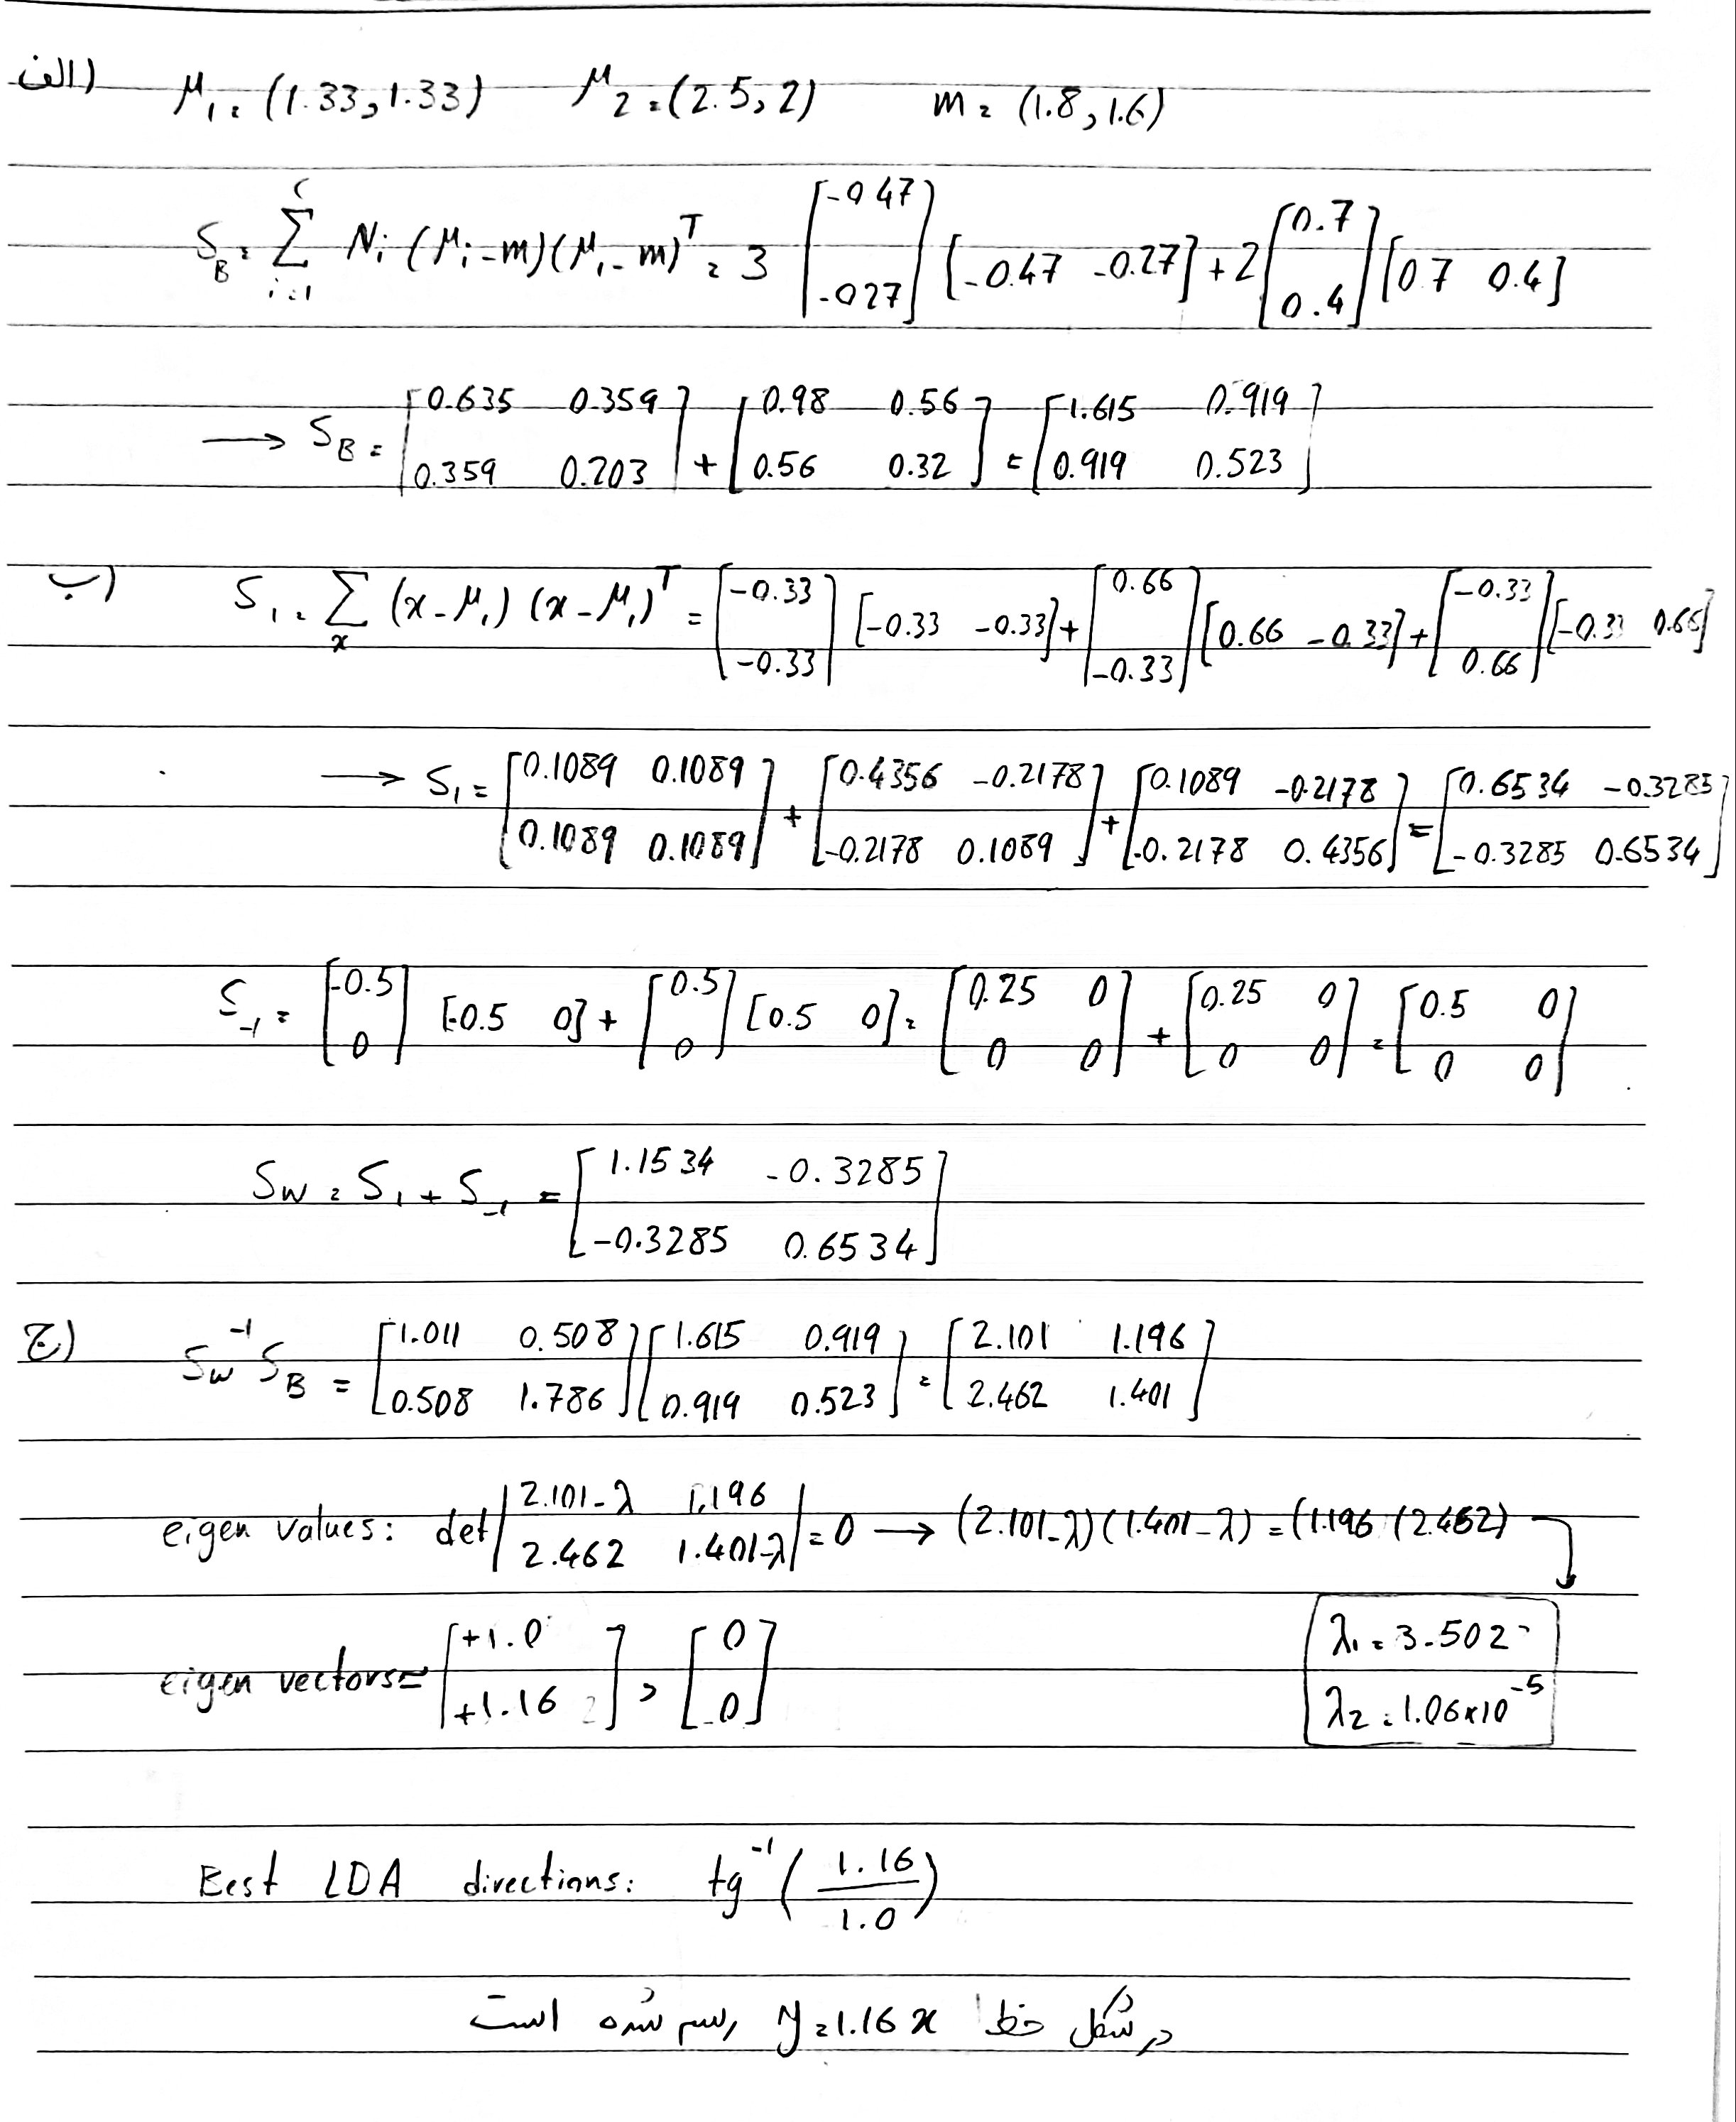
\includegraphics[width=\linewidth]{hand_written/5.jpg}
    \end{center}
\end{figure}
با توجه به شیب خط‌های به دست آمده از قسمت قبل جهت‌های به دست آمده را همراه با داده‌ها رسم می‌کنیم. نقاط قرمز مربوط به $y_{i} = 1$ و نقاط بنفش مربوط به کلاس $y_{i}=-1$ هستند.
\begin{figure}[h!]
    \begin{center}
    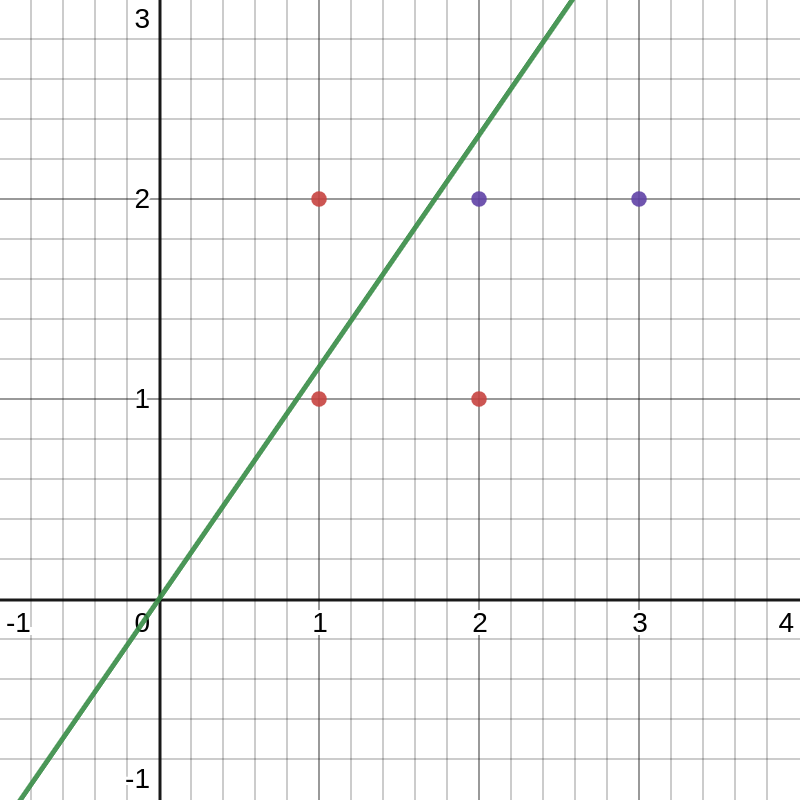
\includegraphics[width=\linewidth]{desmos-graph.png}
    \end{center}
\end{figure}


\newpage
~\newpage
\section*{سؤال شش}
\subsection*{الف}
برای پیاده سازی \lr{SFS} در حلقه \lr{for} بیرونی دو متغیر تعریف می‌کنیم برای یافتن بهترین فیچر جهت اضافه کردن به لیست \lr{selected feature index}. در حلقه \lr{for} درونی که بر روی \lr{i} لوپ می‌زند ابتدا چک می‌کنیم که \lr{i} قبلا انتخاب نشده باشد، سپس بردارهای \lr{x} و \lr{x test} را از روی متغییرهای کلاس و با توجه به ایندکس فیچرهای انتخاب شده تشکیل می‌دهیم و با استفاده از دستورات کتابخانه \lr{scikit learn} دقت آن را بر روی مجموعه تست اندازه گیری می‌کنیم. پس از هر بار ایتریش بر روی متغییر \lr{j} یک ایندکس به زیر مجموعه فیچرها اضافه می‌شود و دقت طبقه بندی آن نیز به لیست \lr{acc list} اضافه می‌شود.
\\
برای رسم نمدار مشابه نمودار مثال از کتابخانه \lr{pandas} و \lr{matplotlib} استفاده شده است. متغییر \lr{th (threshold)} مقداری است که در آن دقت طبقه بندی با زیر مجموعه به دست آمنده بیشتر از ۹۰٪ شود در نمودار با رنگ قرمز رسم شده است. تیک‌های محور \lr{y} نیز لیست بازگردانده شده از متد \lr{forward} می‌باشند. این نمودار در شکل \ref{fig:1} آورده شده است.
\begin{figure}[h!]
    \begin{center}
    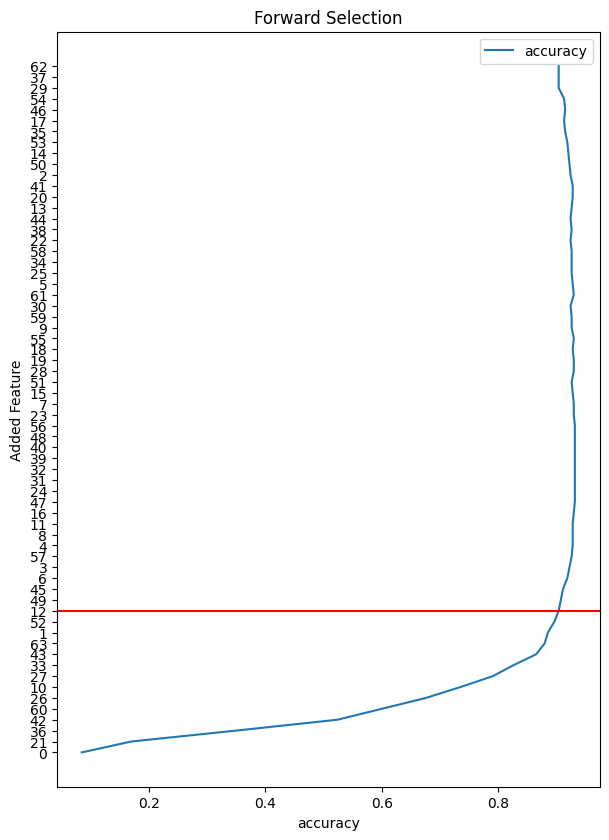
\includegraphics[scale=0.55]{plots/q6_a.png}
    \caption{نتایج اجرای الگوریتم \lr{SFS}}
    \label{fig:1}
    \end{center}
\end{figure}

\subsection*{ب}
این قسمت شباهت زیادی به بخش الف دارد. فقط برای به دست آوردن زیرمجموعه فیچرها از تابع \lr{delete} از کتبخانه \lr{numpy} استفاده می‌کنیم تا بردارهای \lr{x} و \lr{x test} را بسازیم. 
\\
نمودار رسم شده نیز مانند بخش قبل می‌باشد و تنها تفاوت در به دست آوردن مقدار \lr{th} می‌باشد که باید از انتها به ابتدا لوپ زد و مقدار بهینه ترشهولد را به دست آورد. نمودار خواسته شده در شکل \ref{fig:2} نشان داده شده است.
\begin{figure}[h!]
    \begin{center}
    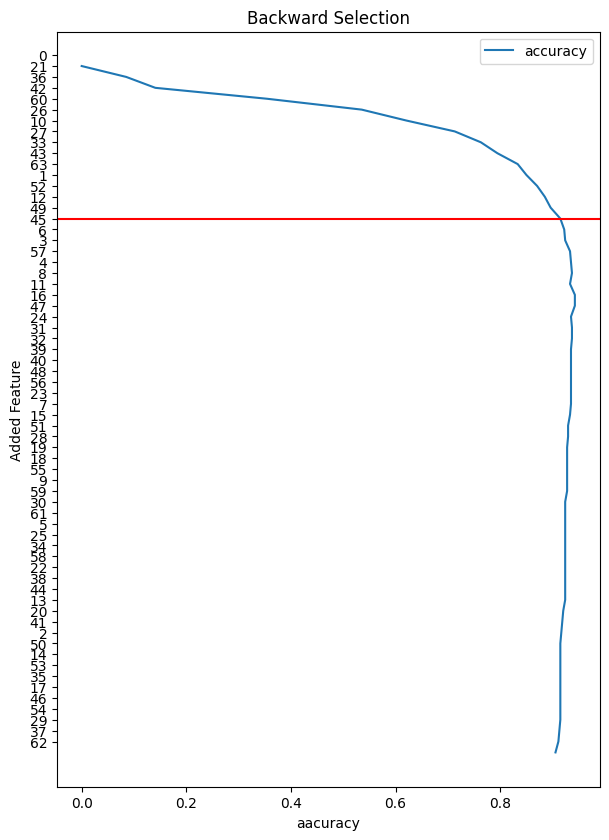
\includegraphics[scale=0.55]{plots/q6_b.png}
    \caption{نتایج اجرای الگوریتم \lr{SBS}}
    \label{fig:2}
    \end{center}
\end{figure}

\newpage
\section*{سؤال هفت}
برای تکمیل تابع \lr{Si} که مقدار \lr{scatter matrix} کلاس \lr{i}ام می‌باشد از رابطه 
$S_{i}=\sum_{\boldsymbol{x} \in D_{i}}^{n}\left(\boldsymbol{x}-\boldsymbol{m}_{i}\right)\left(\boldsymbol{x}-\boldsymbol{m}_{i}\right)^{T}$
استفاده می‌کنیم. در این رابطه $\boldsymbol{m}_{i}$ میانگین داده‌های کلاس \lr{i}ام است. \\
داده‌های ارسال شده در آرگومان ورودی این تابع باید مختص به یک کلاس باشند. جدا سازی داده‌های کلاس‌های مختلف در تابع \lr{Sb} انجام می‌گیرد. در واقع از آرگومان دوم این تابع استفاده نشده است.
\\
برای پیاده سازی تابع \lr{Sw} که \lr{within class scatter matrix} می‌باشد از رابطه
$S_{w}=\sum_{i=1}^{c}S_{i}$
استفاده می‌کنیم.
\\
آخرین تابع که برای محاسبه \lr{LDA} به آن نیاز داریم \lr{Between class scatter matrix} می‌باشد که در تابع \lr{Sb} و به کمک رابطه 
$S_{B}=\sum_{i=1}^{c} N_{i}\left(\boldsymbol{m}_{i}-\boldsymbol{m}\right)\left(\boldsymbol{m}_{i}-\boldsymbol{m}\right)^{T}$
می‌توان آن را محاسبه کرد. در این رابطه $\boldsymbol{m}_{i}$ میانگین نمونه‌های کلاس \lr{i}ام و $\boldsymbol{m}$ میانگین داده‌های تمام کلاس‌ها است. $N_{i}$ نیز تعداد نمونه‌های کلاس \lr{i}ام است.
\\
برای محاسبه ترنسفورمیشن‌های \lr{LDA} مسئله مقادیر ویژه ارائه شده در کلاس درس را باید حل کنیم. بردار $w$ بردار ویژه‌های ماتریس $S_{W}^{-1}S_{B}$ می‌باشد. برای اینکه تابع نوشته شده برای مواردی که ماتریس $S_{W}$ سینگولار می‌شود نیز کار کند از \lr{pseudo inverse} استفاده شده است.
\\
ورودی تمام کلاس‌ها باید آرایه \lr{numpy} باشند. از روی دیتا ست استفاده شده می‌توان مقادیر \lr{data} و \lr{labels} را برای فراخوانی تمام توابع استفاده کرد.
\\
نمودار \lr{seperability} بر حسب تعداد ویژگی‌ها نیز در شکل \ref{fig:3} نشان داده شده است.
\begin{figure}[h!]
    \begin{center}
    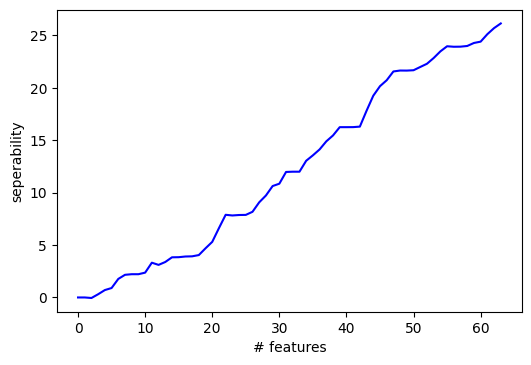
\includegraphics[scale=0.55]{plots/q7_c.png}
    \caption{معیار تفکیک پذیری بر حسب تعداد ویژگی‌های \lr{LDA}}
    \label{fig:3}
    \end{center}
\end{figure}


\newpage
\section*{سؤال هشت}
برای تکمیل تابع \lr{PCATransform} کافی است با دستورات کتابخانه \lr{numpy} ابتدا ماتریس کواریانس داده‌های ورودی را محاسبه کنیم و سپس بردارهای ویژه آن را بر حسب مقادیر ویژه متناظرشان سورت کنیم و در نهایت به تعداد \lr{PC}های خواسته شده  بازگردانیم. در این تابع علاوه بر \lr{PC}های خواسته شده واریانس داده‌های تصویر شده بر روی بردارهای به دست آمده و مقادیر بردارهای ویژه که همان \lr{PC}ها هستند نیز بازگردانده می‌شوند.
\subsection*{الف}
در این قسمت با استفاده از خروجی اول تابع پیاده سازی شده که داده‌های تصویر شده بر روی \lr{PC}ها هستند تصاویر چهره‌ها را بر روی دو کامپننت اول تصویر کرده و در نموداری مانند مثال رسم می‌کنیم. این نمودار در شکل \ref{fig:4} نشان داده شده است.
\begin{figure}[h!]
    \begin{center}
    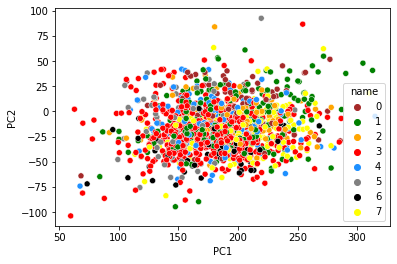
\includegraphics[scale=0.55]{plots/q8_a.png}
    \caption{تصاویر پس از تصویر شدن بر روی ۲ کامپننت اول \lr{PCA}}
    \label{fig:4}
    \end{center}
\end{figure}

\subsection*{ب}
\lr{PCA} یک الگوریتم \lr{unsupervised} است که می‌توان به کمک آن جهت بردارهایی را پیدا کرد که اگر داده را بر روی آن‌ها تصویر کرد به داده‌های در ابعاد پایین تر رسید که بیشترین مقدار واریانس داده‌های اصلی را حفظ می‌کنند. دو این جهت‌ها بردارهای ویژه ماتریس کواریانس هستند و دو کامپوننت اول بردارهای ویژه‌ای هتند که اولین و دومین مقدار ویژه بزرگتر را نسبت به سایر بردارها دارند.
\subsection*{ج}
خروجی دوم تابع پیاده سازی شده در این سؤال نسبت واریانس بیان شده توسط داده‌های تصویر شده بر روی \lr{n} کامپننت اول به صورت تجمعی را نشان می‌دهند. این آرایه \lr{numpy} دقیقاً حاوی داده خواسته شده برای قسمت ب می‌باشد تنها لازم است مقدار ترشهولد را را نیز پیدا کنیم که به سادگی قابل یافتن می‌باشد. این مقدار بر روی نمودار با خط قرمز مشخص شده است. مقدار ترشهولد تعداد کامپوننت‌هایی را نشان می‌دهد که با تصویرسازی داده‌ها بر روی آن‌ها می‌توان ۹۰٪ اطلاعات نمونه‌ها را پس از \lr{dimentionality reduction} نشان داد.
\begin{figure}[h!]
    \begin{center}
    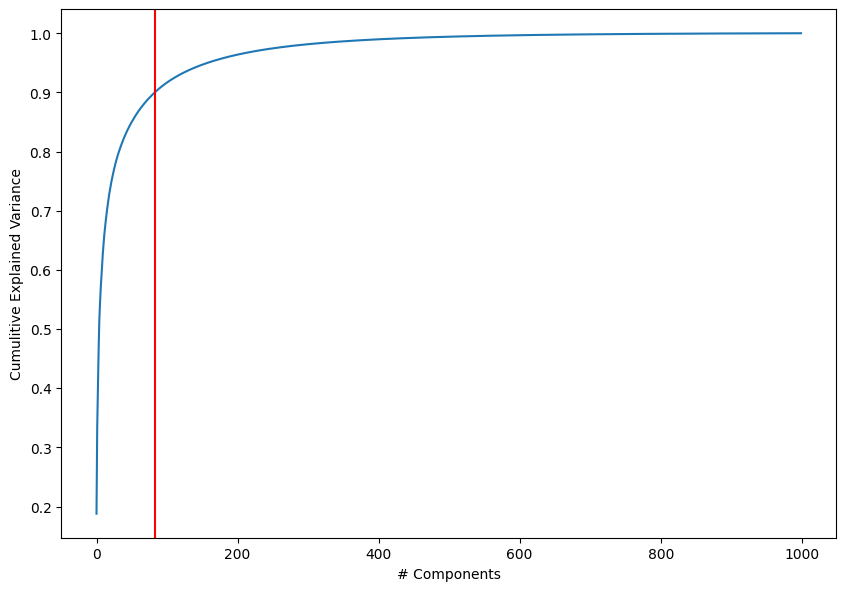
\includegraphics[scale=0.55]{plots/q8_c.png}
    \caption{واریانس داده‌ها پس از انتقال بر روی \lr{PC}ها بر حسب تعداد کامپوننت}
    \label{fig:5}
    \end{center}
\end{figure}

\subsection*{د}
همانند تصاویر رنگی نشان داده شده در مثال داده‌ها را بر روی ۳۰ کامپوننت اول به دست آمده انتقال می‌دهیم و نتیجه تصویر باسازی شده از داده‌های انتقال داده شده در شکل \ref{fig:6} نشان داده شده‌اند.
\begin{figure}[h!]
    \begin{center}
    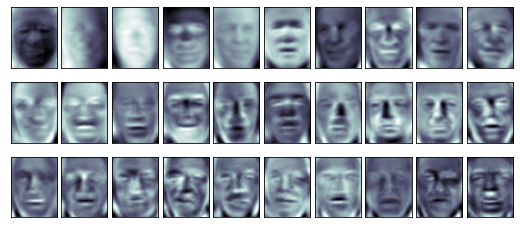
\includegraphics[scale=0.55]{plots/q8_d.png}
    \caption{۳۰ کامپوننت اول}
    \label{fig:6}
    \end{center}
\end{figure}
با وجود اینکه تمام عکس‌های این سؤال \lr{gray scale} می‌باشند، در این بخش برای بهتر دیده شدن با مپ \lr{Blues} نشان داده شده‌اند.\\
قسمت‌هایی از عکس‌ها همان طور که در شکل \ref{fig:6} نشان داده شده است روشن هستند و نوارهایی بر روی تصویر چهره به چشم می‌خورد. همان طور که می‌دانیم پس از تصویر سازی بر روی بردارهای \lr{PC} قسمتی از داده‌ها (چه کم چه زیاد) از بین می‌رود. این قسمت‌های سفید که در تصایر با تعداد کامپوننت کم بیشتر نیز می‌باشند نشان دهنده قسمت‌های از دست رفته نمونه‌ها می‌باشد.

\subsection*{ه}
در این قسمت به ازای مقدار ترشهولد به دست آمده در قسمت ج و همچنین دو مقدار کمتر از آن تصاویر هر هشت نفر انتقال داده شده و مجددا با معکوس انتقال باز گردانده شده از تابع \lr{PCATransform} عکس‌ها بازیابی شده‌اند. نتایج در شکل \ref{fig:7} نشان داده شده‌اند.
\begin{figure}[h!]
    \begin{center}
    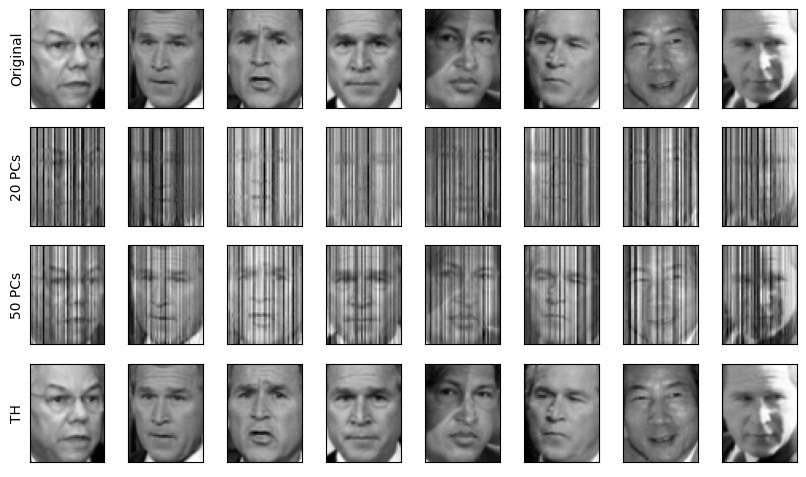
\includegraphics[scale=0.55]{plots/q8_e.png}
    \caption{نتایج \lr{reconstruction} تصاویر پس از انتقال به ازای تعداد مختلفی \lr{PC}}
    \label{fig:7}
    \end{center}
\end{figure}

\end{document}